
	\documentclass{standalone}
	
	\usepackage{tikz, pgfplots, tikz-3dplot}
	\pgfplotsset{compat=1.13}
	   \usepackage{xcolor} 
	   \usetikzlibrary{arrows}
  
  
\begin{document} 


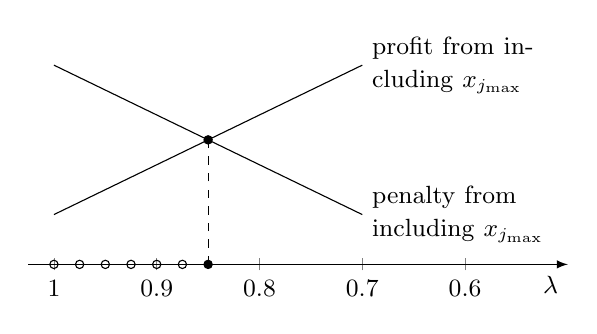
\begin{tikzpicture}
	\begin{axis}[
	xmin=-.5,xmax=10,
	ymin=-1,ymax=8,
%	grid=both,
%	grid style={line width=.1pt, draw=darkgray!10},
%	major grid style={line width=.2pt,draw=darkgray!50},
	axis y line = none,
	axis x line = middle,
	xtick={0,2,4,6,8},
	xticklabels={\small1,\small0.9,\small0.8,\small0.7,\small0.6},
	minor tick num=0,
	axis line style={-latex},	
	xlabel=\small$\lambda$,	
    xlabel style = {yshift=-.5cm},
	]
	\draw[fill=black] (3,2.5) circle (1.5pt);
	\draw[fill=black] (3,0) circle (1.5pt);
	\draw[dashed] (3,0) -- (3,2.5);
	\draw[] (0,0) circle (1.5pt);
	\draw[] (0.5,0) circle (1.5pt);
	\draw[] (1,0) circle (1.5pt);
	\draw[] (1.5,0) circle (1.5pt);			
	\draw[] (2,0) circle (1.5pt);
	\draw[] (2.5,0) circle (1.5pt);
	\draw (0,1) -- (6,4);
	\draw (0,4) -- (6,1);
	\node[anchor=west, text width=2.1cm] at (6,4) {\small profit from including $x_{j_{\max}}$};
	\node[anchor=west, text width=2.5cm] at (6,1) {\small penalty from including $x_{j_{\max}}$};
	\end{axis}
\end{tikzpicture}

\end{document}